
\documentclass[]{spie}

% Package imports go here.
\renewcommand{\baselinestretch}{1.0} % Change to 1.65 for double spacing

\usepackage{amsmath,amsfonts,amssymb}
\usepackage{graphicx}
\usepackage[colorlinks=true, allcolors=blue]{hyperref}
\usepackage{listings}
\usepackage{xcolor}
\usepackage{longtable}
\usepackage{booktabs} % For better looking tables

% Local commands go here.
\newcommand{\aj}{AJ}
\newcommand{\apj}{ApJ}
\newcommand{\apjs}{ApJS}
\newcommand{\procspie}{Proc.\ SPIE}
\newcommand{\pasj}{PASJ}

% Package imports go here.

% Local commands go here.

% See ASPmanual2010.pdf 2.1.4  and ManuscriptInstructions.pdf for more details
%\markboth{auth}{short title}


\newcommand{\docRef}{DMTN-290}
\newcommand{\docUpstreamLocation}{\url{https://github.com/lsst-dm/dmtn-290}}


\begin{document}
%% DO NOT EDIT THIS FILE. IT IS GENERATED FROM db2authors.py"
%% Regenerate using:
%%    python $LSST_TEXMF_DIR/bin/db2authors.py Namespace(mode='spie', noafil=False) 

\author[1]{Angelo~Fausti~Neto}
\affil[1]{Rubin Observatory Project Office, 950 N.\ Cherry Ave., Tucson, AZ  85719, USA}

\author[1]{Frossie~Economou}


\author[1]{Michael~A.~Reuter}


\author[1]{Jonathan~Sick}


\author[1]{Russ~Allbery}


\author[1]{Adam~J.~Thornton}



\title{Sasquatch: Rubin Observatory metrics and telemetry service}

% This can write metadata into the PDF.
% Update keywords and author information as necessary.
\hypersetup{
    pdftitle={Sasquatch: Rubin Observatory metrics and telemetry service},
    pdfauthor={faustinetoa},
    pdfkeywords={}
}

\maketitle


\begin{abstract}
At Vera C. Rubin Observatory, the need to manage metrics and telemetry data efficiently led to the creation of Sasquatch. Sasquatch consolidates our high-frequency telemetry harness, which captures the observatory engineering data, with the science performance metrics measured by the LSST Science Pipelines. Sasquatch utilizes InfluxDB, a time series database to efficiently store and query time-series data. For high availability and data durability we combine InfluxDB Enterprise with Apache Kafka deployed on the Kubernetes platform. The setup at the US Data Facility also enables real-time access of data mirrored from the Summit as well as historical data and provides tools like Chronograf for time series data visualization, Kapacitor for alert management, and the Rubin Science Platform’s notebook environment for data analysis using Python. Currently employed during our System Integration Testing and Commissioning phase, Sasquatch is proving essential as we transition into full operations, offering a scalable solution to our data management challenges.
\end{abstract}



\keywords{Vera C. Rubin Observatory, LSST, Telemetry, Metrics, Time-series Databases}

\section{Introduction}

The Vera C. Rubin Observatory's Legacy Survey of Space and Time (LSST) represents the most ambitious and comprehensive optical astronomy survey ever planned. The LSST will survey the visible sky every few nights, generating a data stream of 20\,TB per night. The survey will produce a 500\,PB dataset over its ten-year lifetime, enabling a wide range of scientific investigations, from studying dark matter and energy to exploring the Solar System \cite{2019ApJ...873..111I}.

The LSST Data Management (DM) team is responsible for developing the LSST Science Pipelines that process the data collected by the LSST. The DM team is also responsible for monitoring the LSST Science Pipelines performance, ensuring that they meet the requirements outlined in the LSST Science Requirements Document (SRD). \cite{LPM-17}

Rubin Observatory also generates a large amount of telemetry data, which is used to monitor the observatory systems' health to diagnose and troubleshoot issues during operations.

This paper describes Sasquatch, a service that is responsible for recording metrics and telemetry data from various subsystems at Rubin Observatory. The paper is organized as follows: Section~\ref{sec:tsd} provides an overview of the science performance metrics and telemetry data produced at Rubin Observatory and its representation as time series data. Section~\ref{sec:arch} describes the Sasquatch architecture. Section~\ref{sec:deploy} presents the Sasquatch deployments at Rubin Observatory. Section~\ref{sec:challenges} dicusses the current challenges and possible solutions. Section~\ref{sec:conc} concludes the paper.

\section{Time series data}
\label{sec:tsd}

In operations, Rubin Observatory will carry out multiple data processing campaigns, including ``first look'' type analysis as images come off the LSST Camera, Prompt Processing, which will process roughly a thousand visits per night, and annual Data Release Processing campaings \cite{LSE-163}. All these processing campaigns will measure science performance metrics to assess the quality of the data products produced by the LSST Science Pipelines. \cite{2019ASPC..523..521B,2022SPIE12189E..0MG} These metrics have a timestamp and are measured across various dimensions understood by the data Butler,\cite{2022SPIE12189E..11J} such as instrument, detector, visit, filter, patch, and tract.

Telemetry is timestamped data and is also measured across various dimensions, such as subsystem, component, and sensor. For example, the forces on each actuator in the Active Optics System of the LSST Primary/Tertiary mirror (M1M3) are measured at 50\,Hz and identified by the actuator number. Similarly, the LSST Camera telemetry data is identified by amplifier, detector, and raft, among other dimensions.

A time series database (TSDB) is optimized for efficiently storing and querying timestamped data, making it ideal for metrics and telemetry data.

The following section describes the Sasquatch architecture, which leverages InfluxDB\footnote{\url{https://www.influxdata.com/time-series-database/}}, a popular TSDB.

\section{Sasquatch architecture}
\label{sec:arch}

Sasquatch\footnote{\url{https://sasquatch.lsst.io}} is designed for high availability and data durability. This is achieved by combining InfluxDB and Apache Kafka\footnote{\url{https://kafka.apache.org}} deployed on the Kubernetes platform. \cite{SQR-029,SQR-068}

InfluxDB can handle high data throughput, making it suitable for writing and querying the high-frequency telemetry data produced by the Observatory Control System (OCS). At USDF we run InfluxDB Enterprise on Kubernetes with a replication factor of two on different data nodes for redundancy. In case of a hardware failure in one of the InfluxDB data nodes, it is still possible to write and query the database.

Apache Kafka is a distributed data streaming platform that is designed for high throughput and fault tolerance. Sasquatch uses the Strimzi operator\footnote{\url{https://strimzi.io}} to deploy Apache Kafka on Kubernetes. Kafka is used to capture telemetry data before writing to InfluxDB. For fault tolerance, Kafka replicates data across multiple brokers in the cluster. Each metric or telemetry topic is configured with a replication factor of three and data durability is ensured by requiring acknowledgment from at least two replicas when writing to Kafka.

Figure 1 shows the Sasquatch deployment at USDF. MirrorMaker2 is the component responsible for mirroring the data from the Summit \cite{SQR-050}. The data is then persisted in the Kafka brokers with a retention period of 72h. Kafka Connect is the component responsible for running the connectors which consume data from the Kafka brokers write to InfluxDB.

\begin{figure}[h]
    \centering
    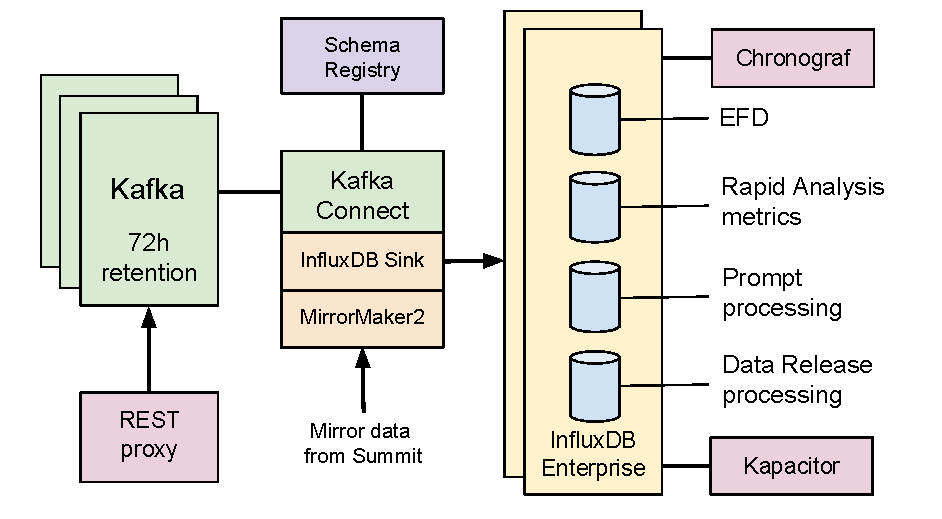
\includegraphics[width=0.8\textwidth]{figures/sasquatch-architecture.pdf}
    \caption{Sasquatch deployment at the US Data Facility.}
    \label{fig:system-architecture}

\end{figure}

Sasquatch implements namespaces to organize and identify different data sources. For example, the namespace \texttt{lsst.sal} is used by Sasquatch to identify Kafka topics produced by the OCS. Kafka Connect then route the data to the corresponding database in InfluxDB, in this example, the Engineering and Facility Database (EFD). Similarly, other namespaces are used to identify metrics data produced by the LSST Science Pipelines and route the data to the corresponding databases in InfluxDB.

\subsection{Sending data to Sasquatch}

Sasquatch uses Avro for the data serialization format and the Confluent Schema Registry (SR)\footnote{\url{https://docs.confluent.io/platform/current/schema-registry/}} to store the Avro schemas and ensure they can evolve safely, whitout breaking the Sasquatch consumers.

Applications connecting to Sasquatch can use native Kafka and SR clients to send data to Kafka. For example, the Kafka producer\footnote{\url{https://ts-salkafka.lsst.io}} that consumes data from the OCS uses the \texttt{confluent-kafka-python} client to send data to Kafka and the Confluent SR client to register the Avro schemas. Avro schemas are created from the XML schemas in the OCS code base\footnote{\url{https://ts-xml.lsst.io}}.

Alternatively the REST Proxy\footnote{\url{https://docs.confluent.io/platform/current/kafka-rest/index.html}} provides a REST interface to Kafka, making it easy to produce and consume messages. The LSST Analysis Tools package measure metrics from the LSST Pipelines outputs uses the REST Proxy to send data to Kafka.

\subsection{Data visualization, alerting, and analysis}

Enabling users to create their own dashboards and alerts is essential for moniroting and troubleshooting the observatory systems, especially during the current System Integration Testing and Commissioning (SITCOM) phase.

Sasquatch uses Chronograf for data visualization, and Kapacitor for alert management. Dahshboards and alert rules ae defined using InfluxQL, a SQL-like query language with a rich set of functions specific to time series data analysis. Alert notifications are sent to specifc channels on Slack to notify the users about a metric deviation from a predefined threshold or the observatory systems health.

Sasquatch is also integrated with the Rubin Science Platform (RSP) \cite{DMTN-082, DMTN-212}. On the RSP at USDF users have access to both real-time and the hitorical data captured by Sasquatch. This integration enables users to perform data analysis in a JupyterLab environment with Python and leverage tools such as Times Square \cite{SQR-062} for publishing parameterized Jupyter Notebooks.

\section{Sasquatch deployments}
\label{sec:deploy}

At Rubin Observatory, Sasquatch is deployed to multiple environments, each with different retention periods, storage capacity, and target audience. Sasquatch deployments are managed by Phalanx\footnote{\url{https://phalanx.lsst.io}}, a kubernetes-based platform for deploying and managing application configutation.

Table 1 shows the different environments where we deploy Sasquatch at Rubin Observatory.

\begin{table}[ht]
    \small
    \centering
    \caption{Sasquatch environments at Rubin Observatory}
    \begin{tabular}{@{}llll@{}}
        \toprule
        \textbf{Environment} & \textbf{Retention Period} & \textbf{Current Capacity} & \textbf{Audience} \\
        \midrule
        Summit & 30 days & 5 TB & Staff at the Summit \\
        USDF & Project lifetime & 60 TB & Project at large \\
        IDF (Google) & 1 year & 30 TB & Project at large (online backup) \\
        Teststands (Tucson \& Base Facility) & 10 days & 1 TB & Developers \\
        \bottomrule
    \end{tabular}
\end{table}

At the Summit, we store data for 30 days, and the main audience for this deployment is the observatory staff.

At the USDF we have requirements to keep the data for the project lifetime and make it available for the project at large. We also deploy Sasquatch on the Google Cloud Platform where we keep the last year of data as an online backup in case users can't access Sasquatch at the USDF.

Finally, we have independent deployments in Tucson, US and at the Base Facility in La Serena, Chile. At the Teststands we record simulated data, and the main audience for these deployments are our developers.

\section{Challenges}
\label{sec:challenges}

We are collecting metrics from LSST Science Pipelines runs on precursor datasets to characterize the performance of the data processing algorithms since early construction \cite{DMTN-091,2022SPIE12189E..0MG}. At the observatory, we started collecting telemetry data in 2019 from the LSST Auxilary Telescope (AuxTel) and from integration tests with the Main Telescope systems such as M1M3 \cite{SITCOMTN-088}, the Telescope Mount Assembly (TMA) \cite{SITCOMTN-121} and the Secondary Mirror (M2) \cite{SITCOMTN-120}.

Even before starting survey operations, we have recorded already 20\,TB of metrics and telemetry data in Sasquatch, with data rates peaking at 565\,GB/week \cite{SQR-085}. With the integration of the LSST Camera into the OCS, planned for this year, we expect the data rates to increase even further.

Table 2 shows the projected storage growth for the EFD database. From the data rates observed so far we estimate the size of the database to increase by 30\,TB/year during survey operations. By the end of the 10-year survey, the final data volume is expected to be around 1\,PB.

\begin{table}[ht]
    \centering
    \caption{Projected storage size for the EFD at USDF by year considering a replication factor of two.}
    \begin{tabular}{@{}lllll@{}}
        \toprule
        \textbf{End of Year} & \textbf{EFD Size} & \textbf{RF} & \textbf{Total Storage} & \textbf{Main Drivers} \\
        \midrule
        2022 & 2 TB & 2 & - & AuxTel \\
        2023 & 15 TB + SM & 2 & 60 TB & M1M3, TMA, M2 + AuxTel \\
        2024 & 35 TB + SM & 2 & 100 TB & MainTel + AuxTel \\
        2025 & 65 TB + SM & 2 & 160 TB & Survey operations \\
        2035 & 0.3-0.5 PB + SM & 2 & 0.7-1 PB & Survey operations \\
        \bottomrule
    \end{tabular}
\end{table}

Managing a database of this size is a challenge. In 2023, we moved from InfluxDB OSS to InfluxDB Enterprise cluster to improve the database scalability and to have access to incremental backup and restore tools, available in the Enterprise product only, but essential for managing the databases in Sasquatch.

At the USDF environment, the InfluxDB Enterprise cluster currently has 2x8-core data nodes with 30\,TB of local SSD storage each and a replication factor (RF) of two for redundancy. As the Sasquatch databases grow in size, we plan on adding more data nodes to the InfluxDB Enterprise cluster to increase the storage capacity while keeping a RF of two. We are actively working with InfluxData support to understand the best practices for scaling the InfluxDB cluster and leveraging the new features available in InfluxDB 3.0, such as storage tiering and the fact that the new version is Kubernetes native.

We use MirrorMaker2 to mirror the data from the Summit to the USDF. With a retention period of 72h in Kafka at the Summit, MirrorMaker2 can automatically recover from network or power outages at USDF. While less frequent, we can recover from outages longer than 72h by restoring data from Summit backups to the USDF InfluxDB instance, however this process still needs automation. In situations where the data is in Kafka but missing in the InfluxDB either at the Summit or USDF environments we can deploy repairer connectors to replay the missing data to InfluxDB. We are also working on improving data consistency by implementing data validation checks in the databases at the Summit ant USDF.

In addition to mirroring data from the Summit to USDF, we also need to support sending metrics computed at USDF back to the Summit in real-time. This requires running another instance of MirrorMaker2 at the Summit to be able to mirror data in both directions. We are currently working on making this feature more reliable in Sasquatch with respect to managing schemas in both environments.

At the Summit environment, the OCS is adopting Apache Kafka for its middleware implementation \cite{2024SPIE13101.59Ftmp, TSTN-033}, which means that the OCS will record commands, events and telemetry data in Kafka in the first place. That puts Apache Kafka into a central role at the Summit, and in principle, we can use the same Kafka cluster for Sasquatch. This change  would simplify the integration of the OCS and Sasquatch at the Summit. For example, the Kafka producers currently used to send data to Kafka won't be necessary, eliminating the data duplication between the OCS and Sasquatch. However, adopting the same Kafka cluster for both the OCS and Sasquatch also brings new challenges. We must configure the OCS Kafka producers properly to achieve the low latency requirements for commands and events topics while prioritizing data durability for telemetry topics.

Finally, we are working on tools to aggregate telemetry \cite{SQR-058} data and expose these data to users in formats like Apache Parquet and VO TAP (Table Access Protocol)\cite{2019ivoa.spec.0927D} to leverage existing data access mechanisms in the RSP.

\section{Conclusion}
\label{sec:conc}

This paper provides a comprehensive overview of Sasquatch. Over the years, Sasquatch's design has evolved significantly, now providing high availability and data durability for metrics and telemetry data. Sasquatch combines InfluxDB Enterprise and Apache Kafka to store and query time series data efficiently. Sasquatch is deployed at multiple environments at Rubin Observatory, each with different retention periods, storage capacity, and target audience.

Sasquatch enables real-time access of data mirrored from the Summit as well as access to historical data at the USDF. Sasquatch also leverages tools such as Chronograf for data visualization and Kapacitor for alert management and is integrated with the RSP notebook aspect for data analysis with Python.

While still facing challenges at the USDF and Summit environments, InfluxDB Enterprise and Apache Kafka offer a solid foundation for Sasquatch. As Rubin Observatory makes its transition into survey operations, Sasquatch, currently employed during the SITCOM phase, is proving to be an essential service.

\vskip 0.4in


% Include all the relevant bib files.
% https://lsst-texmf.lsst.io/lsstdoc.html#bibliographies
\bibliographystyle{spiebib}
\bibliography{local,lsst,lsst-dm,refs_ads,refs,books}

\end{document}
